\documentclass[a4paper,11pt]{article}
\usepackage[osf]{mathpazo}
\usepackage{ms}
\usepackage{natbib}
\usepackage{lineno}
\usepackage{graphicx}
\usepackage{caption}
\usepackage[osf]{mathpazo}
\usepackage[T1]{fontenc}
\usepackage{textcomp}
\modulolinenumbers[5]
\linenumbers
% Eventually this will be generated by the analysis
\def\naccepted{312,069} % from TaxonLookup
\def\ngenbank{92,704}   % Scrubbed genbank
\def\nwoody{40,159}     % Zanne et al
\def\noverlap{28,868}   % Will generated this


\pdfminorversion=3

\makeatletter
\renewcommand{\@biblabel}[1]{\quad#1.}
\makeatother

\title{A simple approach for maximizing the overlap of phylogenetic and comparative data}
\author{
Matthew W. Pennell$^{1,\dag,*}$, Richard G. FitzJohn$^{2,\dag}$, and William K. Cornwell$^{3,\dag}$
}

\date{}
\affiliation{
$^{1}$ Institute for Bioinformatics and Evolutionary Studies, University of Idaho, Moscow, ID 83844, U.S.A. \\
$^{2}$ Department of Biological Sciences, Macquarie University, Sydney, NSW 2109, Australia\\
$^{3}$ School of Biological, Earth and Environmental Sciences, University of New South Wales, Sydney, NSW 2052, Australia\\
$^\dag$ All authors contributed equally\\
$^{*}$ Email for correspondence: \texttt{mwpennell@gmail.com}\\
}

\mstype{Applications Note}
\runninghead{Matching comparative data with phyndr}
\keywords{phylogenetic comparative methods, phylogenetic community ecology, taxonomy, missing data, data imputation}


\begin{document}

\mstitlepage
\parindent=1.5em
\addtolength{\parskip}{.3em}
\vfill

\doublespacing
\section{Summary}
\begin{enumerate}
% RGF: abstract too long (currently ~300 words, aim for 250)
% WKC: now at 251
% MWP: down to 249. boom!!
\item Biologists are increasingly using curated, public data sets to conduct phylogenetic comparative analyses. Unfortunately, there is often a mismatch between species for which there is phylogenetic data and those for which other data is available. As a result, researchers are commonly forced to either drop species from analyses entirely or else impute the missing data.

\item Here we point out a simple solution to increase the overlap while avoiding many of the biases introduced by imputing data.  If some external topological or taxonomic information is available, this can be leveraged to maximize the overlap between the data and the phylogeny without introducing any additional splits. We develop an algorithm that exchanges a species with data for a species without data where all phylogenetic relationships are exactly equivalent. 

\item We have implemented our method in a new R package \textsc{phyndr}, which will allow researchers to apply our algorithm to empirical data sets. It is relatively efficient such that taxon swaps can be quickly computed, even for large trees.

\item To facilitate the use of taxonomic knowledge, at least for plants, we created a separate data package \textsc{taxonlookup}; it contains a curated, versioned taxonomic lookup for land plants and is interoperable with \textsc{phyndr}. 

\item \emph{Synthesis:} Emerging online databases and statistical advances are making it possible for researchers to investigate evolutionary questions at unprecedented scales. However, in this effort species mis-match among data sources will increasingly be a problem; evolutionary informatics tools, such as \textsc{phyndr} and \textsc{taxonlookup}, can help bridge alleviate this issue. 
\end{enumerate}

\vfill

\newpage

\section{Introduction}

Comparative phylogenetic methods can be used to answer a broad range of evolutionary questions \citep{omeara-2012, PennellHarmon}.  At a practical level, doing so generally requires a phylogenetic tree and some set of species-level data; for example data on the species' distribution, demography, species-interactions, physiology, morphology. However, researchers commonly encounter a very simple problem: some species have sufficient genetic data to build a phylogeny but have not been measured for traits of interest; others have been measured for the trait, yet are not placed within the phylogeny.  To gain optimal power from comparative analysis, one generally wants to use as much data from both sources as possible, but the data mis-match prevents this.

This problem has become increasingly common: as the scale of phylogenetic comparative analyses expands --- and fields outside of systematics find creative uses for phylogenetic data --- researchers are increasingly relying on previously published phylogenetic resources, in the form of sequence data and/or phylogenies, and trait data sets. There has been a recent push to assemble, curate, and open up, large collections of data, analogous to \textsc{GenBank}, for this very purpose: \textsc{TreeBASE} \citep{treebase} and \textsc{Open Tree of Life} \citep{OpenTree} for phylogenetic data and \textsc{Encyclopedia of Life} \citep{eol}, \textsc{try} \citep{try}, \textsc{gbif} (\url{www.gbif.org}), and \textsc{compadre} \citep{salguero2015}, among many others, for comparative data.  The availability of phylogenetic data (both original sequence data and phylogenetic trees from published studies) is growing but is far from complete \citep{hinchliff2014}, as is the case for traits. And both of these represent biased samples of life's diversity --- some groups of life and groups of traits have been studied much more intensely than others.

Consider the availability of data for vascular plants, a relatively well-studied group of organisms. There are \ngenbank\ species for which there is currently \emph{any} sequence data in \textsc{GenBank} \citep[As of May 2015 --- accessed using the \textsc{ncbi taxonomy browser};][\url{http://www.ncbi.nlm.nih.gov/Taxonomy/Browser/wwwtax.cgi}]{ncbi-taxonomy}. We compared this list to the \nwoody\ species included in a recent database of plant growth form \citep{Zanne} (Figure \ref{fig:venn}). The key limitation for comparative methods is the area of overlap between the two (Figure \ref{fig:venn}).  While one dataset might be a strict superset of the other, in practice they contain overlap; we found \noverlap\ species represented in both data sets, with more species with trait data having genetic data than ther other way around.

To increase the overlap, aside from both gathering more data and estimating new phylogenies, the researcher is left with few options, all of which involve imputing data in some way. First, it is possible to add unplaced taxa into the phylogeny. If one is willing to assume the monophyly of some higher taxonomic group, it is possible to paste new terminal branches into the phylogenetic tree at approximately the correct location. However, neither the topological position nor the divergence time are known: one must either collapse the higher taxonomic group down to an (artificial) polytomy or randomly resolve relationships. \citet{Kuhn2011} and \citet{ThomasPastis} have suggested using a birth-death process, parameterized from the observed data to randomly resolve polytomies \citep[see also][for a related approach for fossil trees]{Bapst2013} and this approach has been used to fill out trees for comparative analyses \citep{Jetz2012, Price2012, Rolland2014, Jetz2014}. For example, \citet{Jetz2012} produced a phylogeny containing all 9,993 species of birds but 3,323 (33.2\%) of these lacked genetic data and were added in according to a constant rate birth-death process. 

% NOTE[RGF]: What was the reference about community assembly for?
% NOTE[RGF]: This paragraph is really about the danger of inventing
% topology *in general* - separate that out from the polytomy stuff
% and move later
While such an approach may be very useful in some contexts \citep{Kuhn2011}, it may generate often generate biases. A number of simulation studies have investigated this effect \citep{Losos1994, Martins1996, Davies2012, Bapst2014, Rabosky2015} but the rationale is straightforward. If a unresolved clade in a rooted tree contains three taxa then the true phylogeny will only be sampled in 1/3 of random resolutions; more often than not, incorrect sister pairs will be generated. And if a trait of interest has any phylogenetic signal, then the sister species will be appear more divergent than they actually are, thus inflating the apparent rate of evolution. Of course, this problem quickly gets much worse as even more unplaced taxa are considered.

The problem of a mismatch between phylogenetic and trait data could be tackled from the other direction --- some lineages may be included in the phylogeny without a corresponding trait value in the dataset --- using some sort of data imputation method. A number of recent studies have suggested approaches to accomplish this, some using the parameters of a phylogenetic model \citep{Fagan2013, Swenson2014, PEM} and others using a taxonomic sampling model \citep{FitzJohn2014, Sandel2015}. These each have their benefits and drawbacks: using phylogenetic models assumes the observed trait values are a random sample of the distribution of trait values, an assumption that may often be egregiously violated \citep{FitzJohn2014}, whereas taxonomy-based approaches do not make full use of the structure of the phylogeny and require \emph{ad hoc} assumptions about the sampling distribution for the traits. In any case, all of these involve various assumptions about the unknown states and the validity of these may be difficult to assess in many cases.

The strategies described above are potentially useful for increasing the overlap between the tree and the comparative dataset, but as noted, they may have unintended (and in many cases, poorly understood) consequences for downstream comparative analyses. There is, however, a much simpler approach that has to our knowledge been mostly overlooked by biologists: swap unmatched species in the tree with unmatched species in the data that carry equivalent information content. 

Consider a five taxon tree (Figure \ref{fig:algo}A) of the structure $((((\mathcal{A},\mathcal{B}),\mathcal{C}),\mathcal{D}),\mathcal{E})$. If the reconstructed tree contains only taxa $\mathcal{A}$, $\mathcal{C}$, $\mathcal{D}$, and $\mathcal{E}$, such that the resulting tree has the topology $(((\mathcal{A},\mathcal{C}),\mathcal{D}),\mathcal{E})$ but our dataset only contains taxa $\mathcal{B}$, $\mathcal{C}$, $\mathcal{D}$, and $\mathcal{E}$  then trait data from taxa $\mathcal{B}$ can be used in place of trait data for taxa $\mathcal{A}$ without any loss of information. If we simply dropped unmatched taxa, our analysis would only contain 3 taxa, $\mathcal{C}$ and $\mathcal{D}$ and $\mathcal{E}$, whereas if we exchanged $\mathcal{B}$ for $\mathcal{A}$, we would have 4 taxa in our analysis.

This trivial example demonstrates that if external knowledge is available, either in the form of a taxonomy or a more comprehensive topological hypothesis, then it is possible to increase the phylogenetic coverage of the data simply swapping phylogenetically equivalent taxa. Of course, simple taxa exchanges such as the above case are logically straightforward and we suspect that this is commonly done in practice by empirical biologists. However, the problem quickly becomes much more complex as the number of mismatches and potential taxa swaps increases, even more so when there is conflict between the supplied topology or taxonomy and the phylogenetic tree being used for analysis. Here we develop a simple algorithm to generate a set of swaps that maximizes the intersection of the phylogenetic tree and comparative data without inducing any new splits in the tree. We have created an efficient implementation of our algorithm which is available as the R package \textsc{phyndr}. 

\section{Taxon-swapping algorithm}

Our algorithm takes a time-scaled phylogeny, or \emph{chronogram}, a list of species with \emph{trait data} and an externally supplied \emph{guide} --- the guide is distinct from the chronogram. The guide may be either a \emph{topological tree}, a tree containing a more inclusive set of taxa then the chronogram, or else a supplied \emph{taxonomy}. The algorithm differs slightly depending on the type of guide supplied so we deal with these each in turn. We note that technically our algorithm is simply swapping the labels at the tips of the phylogeny but we think it is easier to think of exchanging or swapping taxa, as these are the units of analyses.

% TODO[RGF]: This seems too strong - the maximize bit at least.  Might pay to tone this section down a little.
We conjecture (that is, we suggest without a formal proof) that whether a topological tree or taxonomy is supplied as a guide, our algorithm will always maximize the intersection of the species in the phylogeny and the dataset and will not induce any splits that do not occur in the guide (we refer to such swaps as being \emph{permissible}). In this way, our method is conceptually distinct from approaches that randomly place taxa in a tree given some taxonomic knowledge \citep{Kuhn2011, Jetz2012, ThomasPastis}. 

\subsection{Using a complete toplogy}

Most modern phylogenetic comparative methods are model-based \citep[see recent reviews by][]{omeara-2012, PennellHarmon}, such that branch lengths must be in units of (relative) time for analysis. However, topological information may be available from a larger set of the taxa than included in the estimated chronogram---topological trees may come from large supermatrix phylogenies, supertrees, mega-phylogenies \citep[\emph{sensu}][]{Smithmega}, or more recently, from synthetic tree alignment graphs \citep{Smith2013}, such as those generated by the \textsc{Open Tree of Life} project \citep{OpenTree}. The idea is that the topological tree may be unsuitable for comparative analyses but that it still contains information that may be helpful for comparative analyses using an estimated chronogram. 

All nodes (including tips, nodes without any descendants) can be \emph{complete} or \emph{incomplete}; incomplete nodes are nodes that do not include data that maps \emph{directly} to a species in the chronogram, while complete nodes do.  This definition follows from the fact that we do not consider any swaps for species that have trait data, even if such swaps are permissible given the topology (see below for further comment on this point).

All nodes (including tips) have a \emph{candidate set} of possible matches; these are species with trait data that can go with a given tip.  We store these at nodes where we might prune the tree down to that node.

\begin{enumerate}
\item Drop all species from the chronogram that are not in either the data or in the topological tree as these tips are not saveable.
\item Drop species from the topological tree that are not in the data or the chronogram as they are not informative.
\item Flag all tips that have trait data as \emph{complete}, and all other tips and nodes as \emph{incomplete}.
\item Initialise a \emph{candidate set} for each tip and internal node:
  \begin{enumerate}
  \item for tips that have data, the candidate set is the species name;
  \item for tips without data, the candidate set is the clade within the topological tree that includes the tip and does not include any other species in the chronogram.
  \end{enumerate}
\item In post-order traversal of the chronogram \citep{Felsenstein1973, Felsenstein1981}, for each node:
\begin{enumerate}
  \item if any descendant tip/node is complete then this node is complete; the candidate set remains empty;
  \item otherwise:
\begin{enumerate}
    \item compute the descendants of this node within the chronogram;
    \item compute the most recent common ancestor (MRCA) of these descendants in the topological tree;
    \item compute the descendants of that node within the topological tree;
    \item if any descendant in the topological tree is complete, label this node complete;
    \item otherwise grow the candidate set to include the descendant nodes' candidate set, and then clear the descendant nodes' candidate sets.
\end{enumerate}
\end{enumerate}
This process leaves all species that can be used (are in the union of the chronogram and the data set) in exactly one candidate set, and every node will be complete.
\item Drop all tips in the chronogram with an empty candidate set.
\end{enumerate}

\subsection{Using a taxonomic resource}

It is likely more common that a taxonomic resource is available for the group of interest. Numerous taxonomic resources are available on the web and emerging tools, such as the R package \textsc{taxize} \citep{taxize}, make it possible to interact with them from within R. For the specific examples in this project we also built a tool, the \textsc{taxonlookup} R package, for building a curated taxonomy of vascular plants (see below for details).

For the taxonomic case, the \textsc{phyndr} algorithm works as follows:

Start with a table of taxonomic information; row names are the tip labels in the tree; each column is an increasing taxonomic level (e.g., genus, family, order) that are perfectly nested.  Let a \emph{group} be all species at an instance of a taxonomic level (a group may or may not be a clade in the chronogram).

For each taxonomic level in decreasing order:
\begin{enumerate}
  \item Match species in the chronogram to the data; these species are fixed.
  \item Drop all species that are in the same \emph{group} as species that have data but which do not have trait data.
  \item For each \emph{group} without data, identify if they are monophyletic (i.e., the species in the group form a clade to the exclusion of all other species in the tree).
  \item If the \emph{group} contains at least one member with data:
    \begin{enumerate}
    \item if the \emph{group} is monophyletic, collapse into a single tip;
    \item otherwise, determine if the group can be \emph{made} monophyletic by dropping other groups that do not have data and if so drop those groups and collapse the focal group.
    \end{enumerate}
  \item Otherwise (groups with no data), and if the group survived being dropped above:
    \begin{enumerate}
    \item if the group is monophyletic, collapse into a single tip;
    \item otherwise leave it alone.
    \end{enumerate}
\end{enumerate}

% MWP: [help?]
\subsection{Dealing with topological conflict}

It is important to be explicit about what assumptions we are making when we use a topological tree or taxonomy as a guide. We do not assume that the guide is always correct. Rather, we assume that a group in the topological tree or taxonomy is monophyletic if and only if there is no phylogenetic evidence to contradict this assumption. The \textsc{phyndr} algorithm thus explicitly allows for conflict between the guide and the chronogram. In Figure \ref{fig:algo} we walk through some examples of how our algorithm deals with paraphyletic lineages. It is important to keep in mind that monophyly is assessed using species with trait data --- even if a lineage renders a group non-monophyletic, it will not affect the permissible swaps if it does map to any trait data. We argue that this set of assumptions is rather weak and seems likely to be reasonable for many, but not all, groups of organisms. 

\subsection{Notes on the algorithm}

A number of points are worth considering when applying our algorithm. First, the algorithm does not generate all possible taxon swaps: for lineages that occur in both the tree and the trait data (i.e., those that are considered \emph{complete} in the initial step of the algorithm), we do not consider swaps that exclude the matched species from the final data. If the split $(\mathcal{A,B})$ exists in the guide (whether topological tree or taxonomy) and both taxa $\mathcal{A}$ and $\mathcal{B}$ occur in our data set, but only $\mathcal{A}$ is in the chronogram, it would be consistent with our algorithm to swap $\mathcal{B}$ in for $\mathcal{A}$. However, we have decided to ignore this possibility because it requires making an additional assumption without any gain in information content. (We also note that allowing such swaps would require a more complex algorithm than the one we have proposed.) 

Second, while running analyses across multiple permutations of the datasets may be interesting and useful, this does not account for any uncertainty in topology or branch lengths and can therefore not be considered a ``posterior distribution'' or even a ``pseudo-posterior distribution'' \citep[\emph{sensu}][]{ThomasPastis, Rabosky2015}. For model-based comparative methods, it is better to consider alternative taxa sets as different realizations of the same process. 

Third, our algorithm is restricted to ultrametic phylogenies; taxa are only exchangeable if they are equidistant from their most recent common ancestor, a condition that is only necessarily met when all taxa are sampled at the same time point \citep[see][for more discussion of this point and its implications for models of trait evolution]{SlaterMEE}. So while phylogenetic approaches are becoming increasingly important for analyzing fossil and epidemiological data, alternative strategies will need to be deployed for these cases.

And last, our approach may not be ideal when testing for trait-dependent diversification \citep[e.g.,][]{Maddison2007, FitzJohn2012} or correlations between rates of diversification and rates of trait evolution \citep[e.g.,][]{Rabosky2013, Rabosky2014} (see \citealt{PennellPE} for a discussion of the distinction between these two types of analyses). Dropping tips without any data, which is a step of the \textsc{phyndr} algorithm, will tend to push the terminal nodes rootwards and thus bias estimation of diversification rates. Essentially, this is similar to biases introduced by ``representative'' sampling, in which phylogenies are built using representatives of major taxonomic groups \citep{Hohna2011, Stadler2013}. The sampling regime introduced by \textsc{phyndr} is somewhat different from that studied by \citet{FitzJohn2009}, in which all taxa in the phylogeny and assign unknown trait values to species without data, and therefore an alternative correction is needed for this case.  

\section{phyndr R package}

We have implemented our algorithm in a new R package \textsc{phyndr}. It can be downloaded from the CRAN repository (\url{http://cran.r-project.org/web/packages/phyndr/index.html}) and the development version is available on GitHub (\url{https://github.com/richfitz/phyndr}). \textsc{phyndr} relies on the \textsc{ape} \citep{ape} tree structure and \textsc{diversitree} \citep{FitzJohn2012} tree manipulation functions. \textsc{phyndr} contains two primary functions \texttt{phyndr\_topology}, and \texttt{phyndr\_taxonomy} that use topological trees and taxonomies, respectively, as guides. (Generic names can be stripped from taxon labels and used to create a genus-only taxonomy with the function \texttt{phyndr\_genus}.) 

The \texttt{phyndr\_} functions each generate a \texttt{ape::phylo} object with the taxon names relabeled where possible. If multiple relabelings for a given taxa are permissible, one is randomly selected by default but the others are stored in the returned object so that users can generate sets of trees that match to different subsets of the trait data. Note that given the combinatorial nature of the problem, the number of potential relabelings can grow rather quickly and returning the full set may not be possible in R. Furthermore, the encoding of alternative taxon labels could be included in a NeXML file \citep{nexml}, using the \textsc{RNeXML} package \citep{rnexml}, to be stored and distributed along with the tree structure.

\section{taxonlookup R package}

The \textsc{taxonlookup} R package dynamically builds a taxonomic lookup for vascular plants from three canonical sources: \textsc{The Plant List} \citep{ThePlantList}, \textsc{APWeb} \citep{apweb}, and a recently published higher taxa lookup table \citep[][compiled by D.C. Tank, J.M. Eastman, J.M. Beaulieu, W.K. Cornwell, P.F. Stevens, and A.E. Zanne]{ZanneDryad}.  This will keep the taxonomy resource up-to-date as systematic information improves through time.  It is freely available on CRAN  (\url{http://cran.r-project.org/web/packages/taxonlookup/index.html}) and on GitHub (\url{https://github.com/wcornwell/taxonlookup}); currently only vascular plants are covered by this resource, but it could be extended to cover other taxa. For \textsc{taxonlookup} we have tried to sort out conflicts and errors in the web-based resources and the package provides output that is can be easily used in conjunction with \textsc{phyndr}.

\section{An example}

As a use-case, we applied our algorithm to a recently published time-calibrated phylogeny of vascular plants \citep{Magallon2015} and a database of plant growth form \citep{Zanne}. The \citet{Magallon2015} chronogram contains 798 taxa and many of these were chosen as single representatives of major groups (thus making it an ideal situation for applying our algorithm). Dropping species for which there was not an exact match between the phylogeny and the trait data would leave us with only 238 taxa---540 data points are lost!

To improve the overlap, we use \textsc{phyndr} in conjuction with the taxonomic table in \textsc{taxonlookup} as follows (assuming we have already loaded a \texttt{phy} [an \texttt{ape::phylo} object] and \texttt{dat} [a \texttt{data.frame} with rownames equal to the species names] objects into the workspace):
\begin{flushleft}
We can get the entire taxonomy table from \textsc{taxonlookup} using \texttt{plant\_lookup}:\\
\texttt{library(taxonlookup)}\\
\texttt{tax\_all <- plant\_lookup()}\\
\bigskip
But for our algorithm, we only need taxonomy for all species in tree and data, which can be obtained with the function \texttt{taxonlookup::plant\_lookup}:\\
\texttt{spp <- unique(c(phy\$tip.label, rownames(dat))}\\
\texttt{tax\_spp <- lookup\_table(spp, by\_species=TRUE)}\\
\texttt{tax\_spp <- tax\_spp[,c(``genus'', ``family'', ``order'')]}\\
\bigskip
We can then run \textsc{phyndr} to get all permissible taxon swaps:\\
\texttt{library(phyndr)}\\
\texttt{phyndr\_taxonomy(phy, rownames(dat), tax\_spp)}\\

\end{flushleft}
This gives us a comparative data set including 769 species; we have recovered a match for all but 29 of the previously unmatched taxa (Figure \ref{fig:plant-tree}). (Code to reproduce this example can be found at \url{https://github.com/mwpennll/phyndr-ms}.) Similarly, we could have used \texttt{phyndr\_topology} and replaced the taxonomic table with a previous topological hypothesis for this group.
 

\section{Closing remarks}

In recent years, there have been increasing coordination to assemble different species-level data types including observations, traits, genes, and phylogenies \citep{Parr2012}.  These data sources, while already large and growing, do not overlap completely, and are unlikely to do so for the foreseeable future.  As such, any type of synthetic research involving two data sources have a matching problem, and this matching problem will be increasingly common moving into the future.  We sought to find a method that increases overlap while not introducing a new source of error.  On one level, our method is rather obvious. If one is willing to assume that when a node it is present in both the chronogram and a topological or taxonomic hypothesis it can be taken as correct, our method follows from a basic property of ultrametric trees: at any node, the labels of the daughter clades are interchangeable. However, for large, complex topologies with varying degrees of conflict, it is challenging to reason through all permissible label swaps. And even for relatively simple scenarios, automating the process is non-trivial. We believe that \textsc{phyndr} will enable empirical biologists to efficiently and reliably make the most of their data.

A generalised comparative methods workflow consists of the following steps:  1) match exact names; 2) match misspelled and outdated names; 3) substitute close relatives; 4) substitute wherever you can without introducing error; 5) prune the tips with missing data; 6) do analysis.  In recent years the tools for some of these steps have improved.  For example, step (2) is much easier with \textsc{taxize} \citep{taxize}, \textsc{Taxonstand} \citep{cayuela2012} and other tools.
%
% Both GNR and TNRS use outdated names lists, if you use either with taxonlookup there will be synonymy chaos..so we probably shouldn't propose that as a workflow..
% Taxonstand queries The Plant List, so at least then we're tied to one canonical data source.  
%online services, such as the \textsc{Global Names Resolver} (\url{http://resolver.globalnames.org/}) and the \textsc{iPlant Taxonomic Name Resolution Service} (\url{http://tnrs.iplantcollaborative.org/index.html}; \citealt{tnrs}).  
%
Our taxonomic package \textsc{taxonlookup}, built upon open datasets from \textsc{The Plant List} \citep{ThePlantList}, \textsc{APWeb} \citep{apweb}, and \textsc{Open Tree of Life} \citep{OpenTree}, and the algorithms in \textsc{phyndr} are aimed to maximize effectiveness of steps (3) and (4). We think that our tools will help biologists get the most of their data and be a generally applicable addition to many different comparative methods workflows.

\section{Acknowledgements}
We thank the members of the Tempo and Mode of Plant Trait
Evolution working group for stimulating discussions of this problem. In particular, we are grateful to Luke Harmon, Josef Uyeda, and Eliot Miller for advice and comments. We thank Scott Chamberlain and the ROpenSci organization for techincal assistance with the taxonomic resources. This work was supported by the National Evolutionary Synthesis Center
(NESCent), NSF \#EF- 0905606, Macquarie University Genes to Geoscience
Research Centre through the working group. MWP was supported by a NSERC postgraduate fellowship. This work was also supported by a NSF grant awarded to Luke J. Harmon (DEB 1208912) at the University of Idaho. 


\clearpage

\bibliographystyle{jecol}
\bibliography{phyndr.bib}

\begin{figure}[p]
\includegraphics{figs/venn}
\caption{Overlap (purple) of species with recognized names (yellow), trait data in the global woodiness data base \citep[blue][]{Zanne, FitzJohn2014}, and which have sequences deposited in \textsc{GenBank} (orange) (All, as of May 2015). The total diversity of plants (grey) is not known.}
\label{fig:venn}
\end{figure}

\begin{figure}[p]
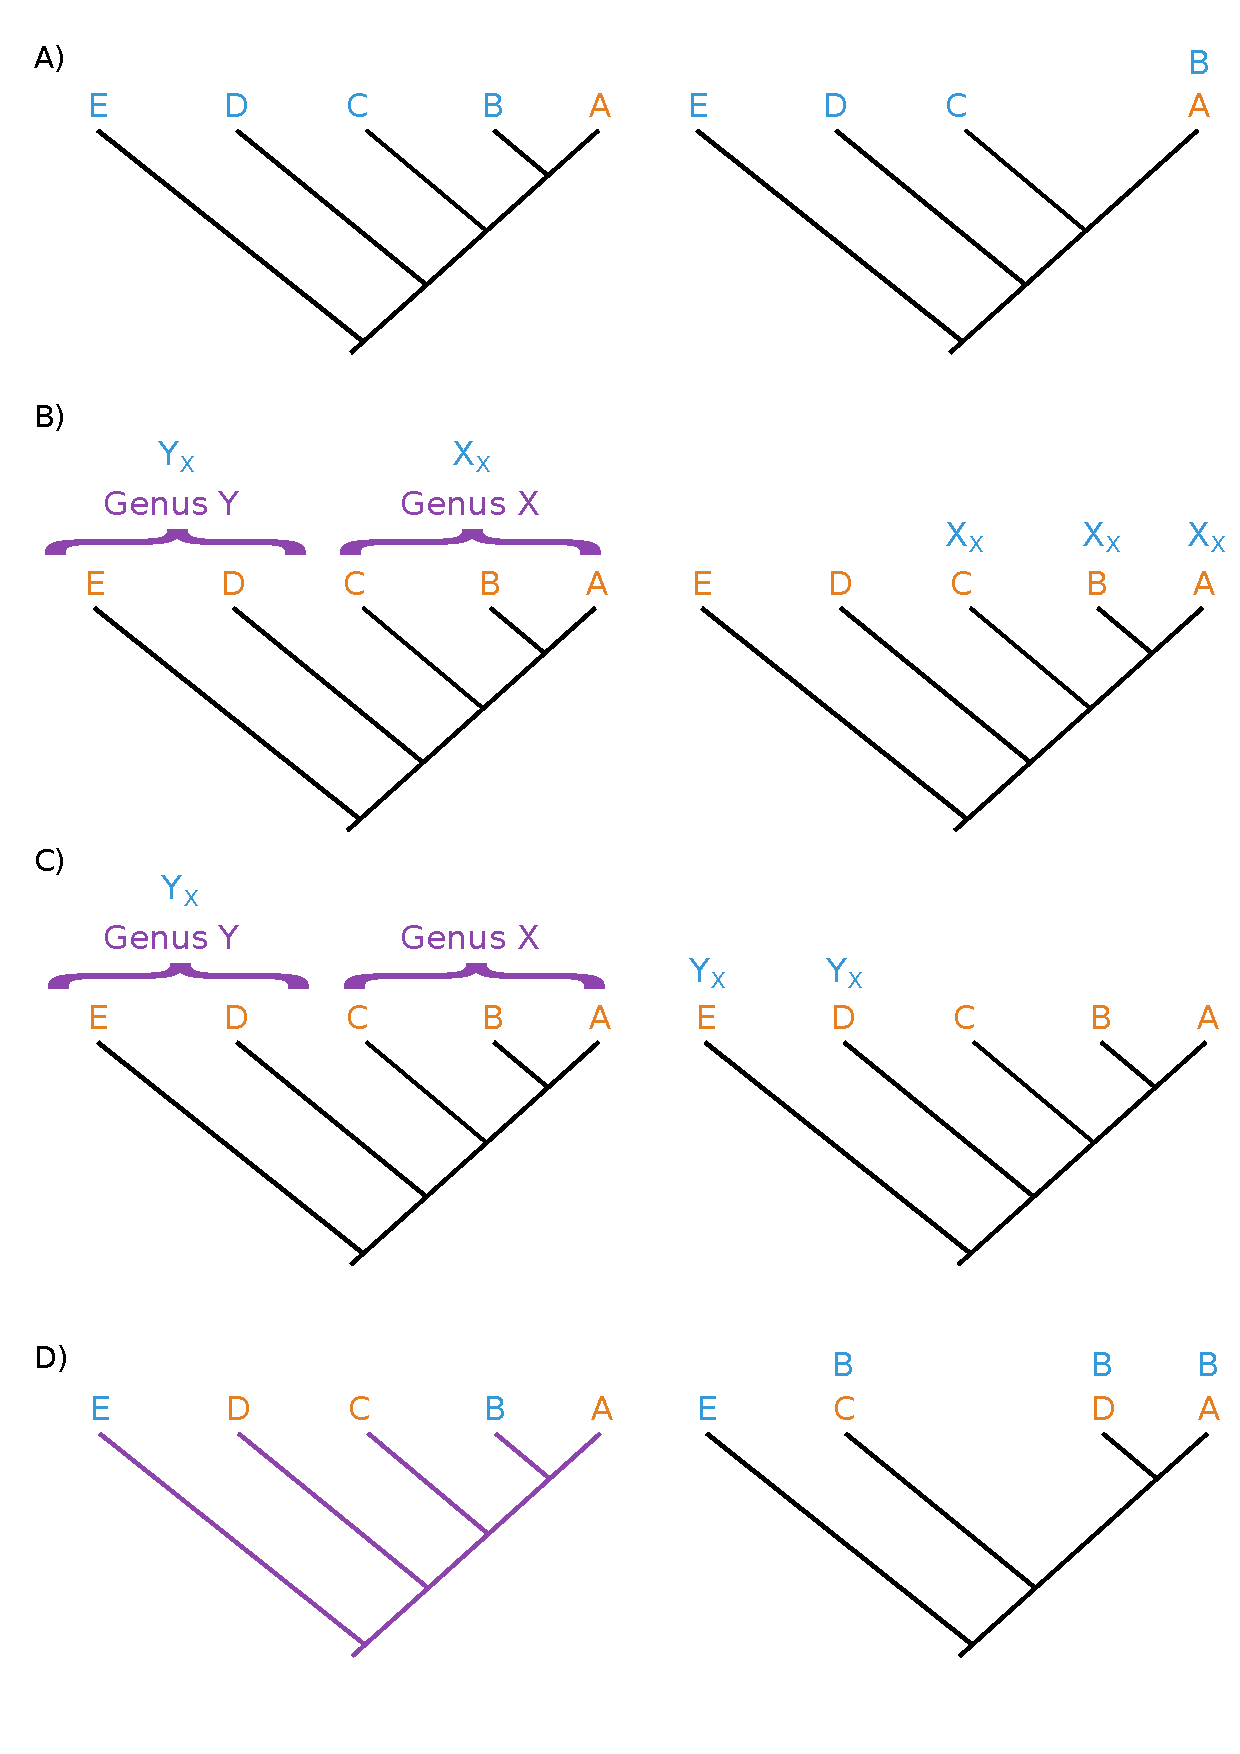
\includegraphics[scale=0.7]{figs/algo-description}
\caption{}
\label{fig:algo}
\end{figure}

\addtocounter{figure}{-1}
\begin{figure} [p]
  \caption{A few examples illustrating the reasoning behind our algorithm. Blue labels indicate species with trait data and orange indicates those without. Panel A) Because they are sister species, lineages A and B are interchangeable; if we have trait data for one and phylogenetic data for the other, the labels can be swapped (as indicated by the label B over A on the right side). The challenge with incorporating taxonomic information (purple) is that the phylogenetic hypothesis may suggest that named groups are paraphyletic. If the placement of Genus X implies that Genus Y is paraphyletic, then label swaps are only permissible in Genus X if trait data is available for representatives of both X and Y (Panel B). However, if trait data is only available for a representative of genus Y, the label of this lineage can be exchanged with any other member of the genus as all tips from Genus X will be dropped. If one has a topological tree (purple branches; Panel D), a similar principle to the taxonomic case can be applied. Even though lineages C and D are in different positions in the topological tree and the chronogram, because no members of the clade (A,C,D) have data, one can swap in species B for any of these lineages without inducing any splits in the tree.}
\end{figure}

\begin{figure}[p]
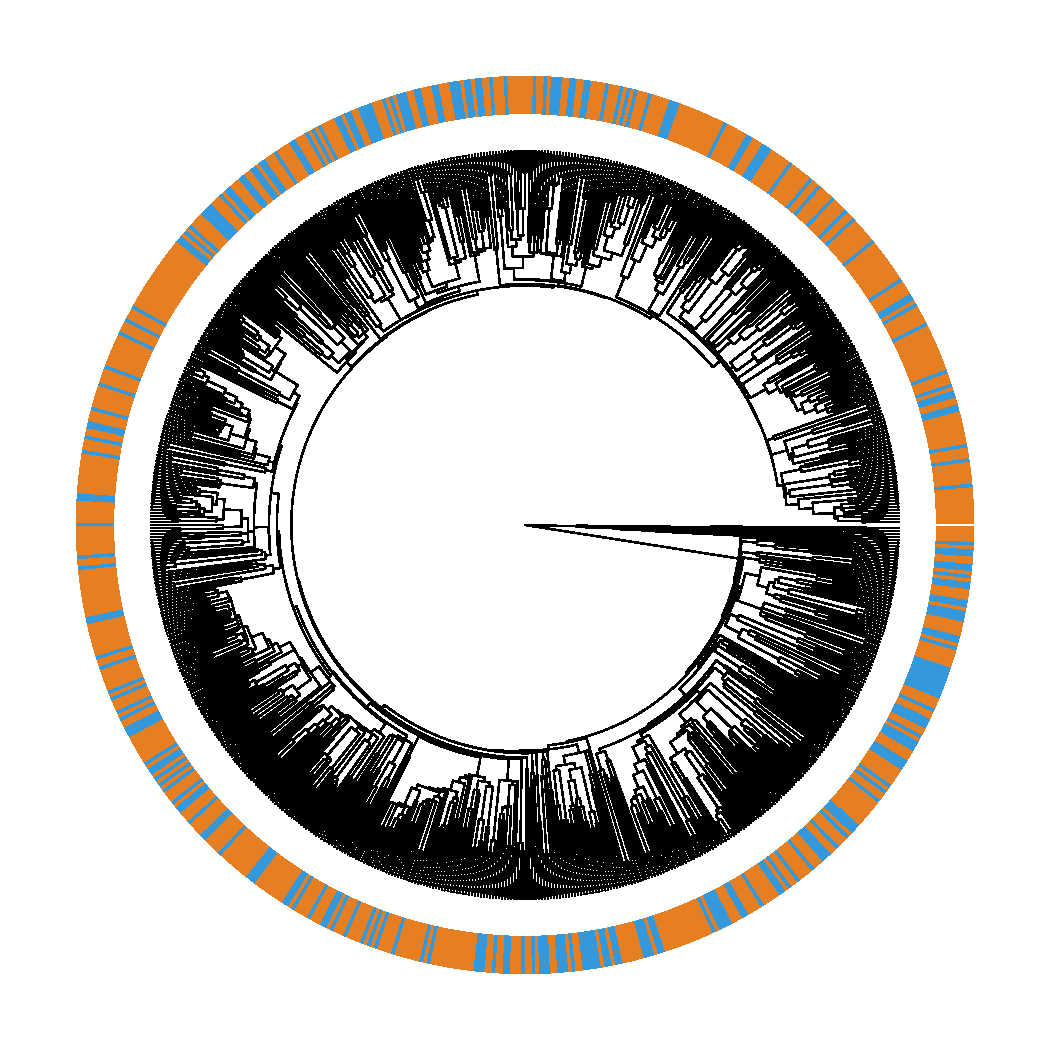
\includegraphics[scale=0.75]{figs/tree-fig-temp}
\caption{The phylogenetic tree of vascular plants from \citet{Magallon2015} after performing label swaps with \textsc{phyndr} using the taxonomic resources in \textsc{taxonlookup}. The original phylogeny contained 798 taxa, only 238 (blue) of which were also in the growth form database. Using \textsc{phyndr}, we were able to find matches for 531 additional taxa (orange).}
\label{fig:plant-tree}
\end{figure}

\end{document}
